\documentclass[conference]{IEEEtran}
\IEEEoverridecommandlockouts
% The preceding line is only needed to identify funding in the first footnote. If that is unneeded, please comment it out.
\usepackage{cite}
\usepackage{amsmath,amssymb,amsfonts}
\usepackage{algorithmic}
\usepackage{graphicx}
\usepackage{textcomp}
\usepackage{xcolor}
\usepackage{color}
\usepackage{url}
\def\BibTeX{{\rm B\kern-.05em{\sc i\kern-.025em b}\kern-.08em
    T\kern-.1667em\lower.7ex\hbox{E}\kern-.125emX}}

\hyphenation{op-tical net-works semi-conduc-tor}
\newcommand{\xslnote}[1]{{\bf\color{red}[ #1 -- SHERRY ]}}


\begin{document}

\title{Distributed simulation of macroscopic \\ traffic models for large networks}

\author{\IEEEauthorblockN{Gabriel Gomes}
\IEEEauthorblockA{\textit{dept. name of organization (of Aff.)} \\
\textit{name of organization (of Aff.)}\\
City, Country \\
email address}
\and
\IEEEauthorblockN{Juliette Ugirumurera}
\IEEEauthorblockA{\textit{dept. name of organization (of Aff.)} \\
\textit{name of organization (of Aff.)}\\
City, Country \\
email address}
\and
\IEEEauthorblockN{Xiaoye Li}
\IEEEauthorblockA{\textit{dept. name of organization (of Aff.)} \\
\textit{name of organization (of Aff.)}\\
City, Country \\
email address}
}

\maketitle

\begin{abstract}
THIS IS THE ABSTRACT
\end{abstract}

\begin{IEEEkeywords}
XXX, YYY, ZZZ
\end{IEEEkeywords}

\IEEEpeerreviewmaketitle

\section{Introduction}
% Simulation speed is crucial when traffic simulation is used in real-time traffic management or traffic forecasting applications \cite{lee2002framework}.
\IEEEPARstart{R}{ecent} years have seen significant technological changes in transportation with the advent of shared-mobility like Uber and Lift, electric vehicles, and autonomous. There is a need for government agencies and industry to understand the impact of wide-spread adoption of these new technologies on the large-scale transportation system. This in turn requires tools to model the transportation system at the city scale, requiring large computing and memory resources. Parallel computation and modern supercomputers provide the power and memory to handle such large-scale traffic simulation. They also enable running thousands of parallel simulations that can answer future what-if scenarios.
Traffic simulation developers have adopted parallel computation techniques for traffic simulation of large networks. On a multiprocessor shared-memory computer, parallel simulation takes advantage of the computer's many processors to execute tasks in parallel. In this case, the simulation speed-up is limited by the number of processors on the one computer. On a multiprocessor distributed-memory computer system, parallel simulation can use processors on multiple computers while communicating over a message passing system. This paper describes such an approach for a fluid-based traffic simulation models. We begin by reviewing previous efforts, most of which have focused on vehicle-based (microscopic and mesoscopic) models. 

% We should have a section that show when to use macroscopic simulation and why it is needed at large-scale too. 

\subsection{Related Works}

\begin{table*}[htbp]
\centering
\begin{tabular} { | l | p{25mm} | p{80mm}| } 
	\hline
	\hline
	\textbf{Software} & \textbf{Traffic Model} & \textbf{Parallel Method}\\ \hline
	Paramics \cite{cameron1996paramics} and FastTrans \cite{thulasidasan2009accelerating}    & Microscopic Model & Parallel computation on distributed-memory computer with MPI for inter-core communication \\ \hline
	TRANSIMS \cite{robertson1969transyt}     & Microscopic Model & Parallel computation on distributed-memory computer with MPI and PVM for inter-core communication \\ \hline
	AIMSUN \cite{ferrer1993aimsun2}, SEM-Sim \cite{aydt2013multi} and MEgaffic \cite{osogami2012research}     & Microscopic Model & Multi-Threading \\ \hline
	SUMO \cite{behrisch2011sumo}    & Microscopic Model & Multi-threading for routing \\ \hline
	BEAM \cite{aboutBeam}    & Microscopic Model & Akka library \\ \hline
	Dynemo \cite{nokel2002parallel}  & Mesoscopic Model & Network distribution through master-slave parallelization \\ \hline
	Mobiliti \cite{chan2018mobiliti}     & Mesoscopic Model & Parallel discrete event with GASNet \\ \hline
	\cite{xu2014mesoscopic,song2017supporting}and \cite{strippgen2009multi}     & Microscopic Model & Parallel computation on GPUs \\ \hline
	\cite{chronopoulos1998real}     & Macroscopic Model & Distribution of freeway sections on multiple processes of a nCubes2 distributed-memory parallel computer \\ \hline
	\cite{johnston1999parallelization}     & Macroscopic Model & Distribution of highway segments on multiple processes of a Cray T3W distributed-memory parallel computer \\ \hline
	OTM     & Macroscopic Model & Domain decomposition of network with highway, arterial and local roads. Use MPI for inter-process communication \\ \hline
\end{tabular}
\caption{Softwares for Dynamic User Equilibrium}
\label{tab:softwares}
\end{table*}

%\xslnote{Define micro-, meso- and macro simulations.}

Since Greenshield presented the first traffic model in 1934 \cite{greenshields1934photographic}, three main traffic model categories have emerged: microscopic models, macroscopic models and mesoscopic models. Microscopic models traffic by representing the behavior and interaction of individual vehicles. Macroscopic models describe traffic as a continuum flow with density, flow and speed parameters. Mesoscopic models combine characteristics of macroscopic and microscopic models: traffic movement is represented in aggregate way, while the rules of behavior are modeled per individual vehicles \cite{van2015traffic}. Traffic simulation software tools can also be grouped into microscopic, macroscopic and mesoscopic simulators depending on the model they implement. 

Most prominent traffic simulation software that have parallel computation implementations are microscopic traffic simulators. Parallel Microscopic Simulation (Paramics) \cite{cameron1996paramics} microscopic simulator was implemented on a the T3D parallel computer with Message Passing Interface (MPI) for inter-processor communication. FastTrans \cite{thulasidasan2009accelerating} and TRansportation ANalysis and SIMulation System (TRANSIMS) \cite{nagel2001parallel} microscopic simulators use parallel computation on distributed-memory
%multi-core \xslnote{In 1996, there is no multi-core machine.} 
computer systems by dividing the road network into multiple sub-networks that are distributed among processes running on the multiple computing cores; FastTrans use MPI library to share boundary information among processes, while TRANSIMS can support
both MPI and Parallel Virtual Machine (PVM) communication interface. The Advanced Interactive Microscopic Simulator for Urban and Non-Urban Networks (AIMSUN) \cite{ferrer1993aimsun2}, Scalable Electro-Mobility Simulation (SEM-Sim) \cite{aydt2013multi}, and the IBM Mega Traffic Simulator (MEgaffic) \cite{osogami2012research} implement parallel computation through the multi-threading approach, which enables to run multiple threads in parallel to update simulated agents simultaneously. The Simulation of Urban Mobility (SUMO) microscopic simulator
exploits multi-threading parallel computation for vehicle routing,
but the rest of simulation is single-core \cite{behrisch2011sumo}.
The Behavior, Energy, Autonomy and Mobility (BEAM) simulator \cite{aboutBeam} extends the Multi-Agent Transportation simulator (MATSIM) \cite{horni2016multi}, which is a microscopic traffic simulator. BEAM incorporates parallel computation via the Akka \cite{akka} library, which implements the Actor Model computation \cite{actorModel}. 

 For mesoscopic traffic simulation, N{\"o}kel and Schmidt present a parallel implementation for the Dynemo mesoscopic simulator that uses a master-slave parallelization. The master process initializes the simulation and distributes the network among multiple slave processes. The slave processes calculates the spatial motion of the vehicles on their sub-networks and shares boundary information through PVM communication interface. Mobiliti \cite{chan2018mobiliti} is another mesoscopic traffic simulator that model links as agents and vehicles as events. It uses the parallel discrete event paradigm and a GASNet communication layer to enable parallel computation on high performance computing resources or clusters.The POLARIS mesoscopic simulator \cite{auld2016polaris} exploits parallel computation via multi-threading. References  \cite{xu2014mesoscopic,song2017supporting,strippgen2009multi} present mesoscopic traffic simulation frameworks that take advantage of parallel computation on graphics processing units (GPUs). 

On the other hand, parallel computation has not been applied extensively in macroscopic traffic simulation. Work \cite{chronopoulos1998real} present a parallel implementation of a continuum traffic flow model for freeway modeling on a nCubes2 hypercube distributed-memory parallel computer, where freeway is partitioned into equal segments and assigned to different processors. Each processor sends the calculated density, speed and volume on its segment to processors handling adjacent segments. Similarly, Johnston and Chronolopoulus \cite{johnston1999parallelization} describe a parallelization of lax-momentum traffic model for a highway that divided the highway into equal segments assigned to different processors. The simulation was run on Cray T3E 
%\xslnote{I know about T3D, T3E, but not T3W}
distributed-memory computer system. Though \cite{chronopoulos1998real} and \cite{johnston1999parallelization} use parallel computation for macroscopic traffic simulation on distributed-memory computers, they are focused on freeway simulation. In addition, the performed simulation studies were on small networks (18 to 20 mile freeway) and were executed on older computer systems.

The work we present here is based on the Open Traffic Models simultor. OTM is a full-featured traffic simulator that has in the past been used in single-process environments. OTM is a \textit{hybrid} simulator, in the sense that it incorporates multiple (macroscopic, mesoscopic, and microscopic) models which can be combined arbitrarily on a single network. It also supports multiple road geometries (turn pockets, managed lanes on freeways, etc.), multiple vehicle types, and a variety of traffic control systems (traffic signals, variable speed limits, onboard information systems, etc.). Here we focus on the parallelization of the macroscopic model only. This is both because there are many high quality distributed implementations of vehicle-based models, and because it avoid some of the complexities of asynchronous updates that occur in vehicle-based model.


\section{Methodology}
The full mathematical description of the model can be found in [XXX]. The description provided here omits certain details, but is sufficient to understand the inter-process communication that enables distributed simulation. The model is in the class of \textit{cell transmission} models first introduced by Daganzo in XXX. Since then there have been many extensions and improvements to the CTM, incorporating multiple lanes, non-triangular fundamental diagrams, etc. The CTM model that is implemented in OTM is adapted to an underlying representation of the road that is shared among 
all models in the hybrid simulation environment. As with most traffic simulators, there is a high-level graph (links and nodes) which provides the connectivity between roads at intersections. Each link (i.e. a segment of road between two junctions) has an internal geometry consisting of multiple lanes, lane pockets, and possibly a managed lane with access gates (in the case of a freeway link). There can also be sensors and control devices within the link. 

The relations between lanes that enter and exit a junction are defined by \textit{road connections}. A road connection indicates which lanes in an upstream link can turn into which other lanes in a downstream link. For example, a road connection may indicate that vehicles must be in the outer two lanes of the freeway in order to reach the offramp. The road connections the leave a link can be used to group the lanes of the link that travel at similar speeds. These form the \textit{lane groups}; in our previous example, the two outer lanes constitute a lane group, and the remaining inner lanes are another. 

\begin{figure}[h!]
    \centering
    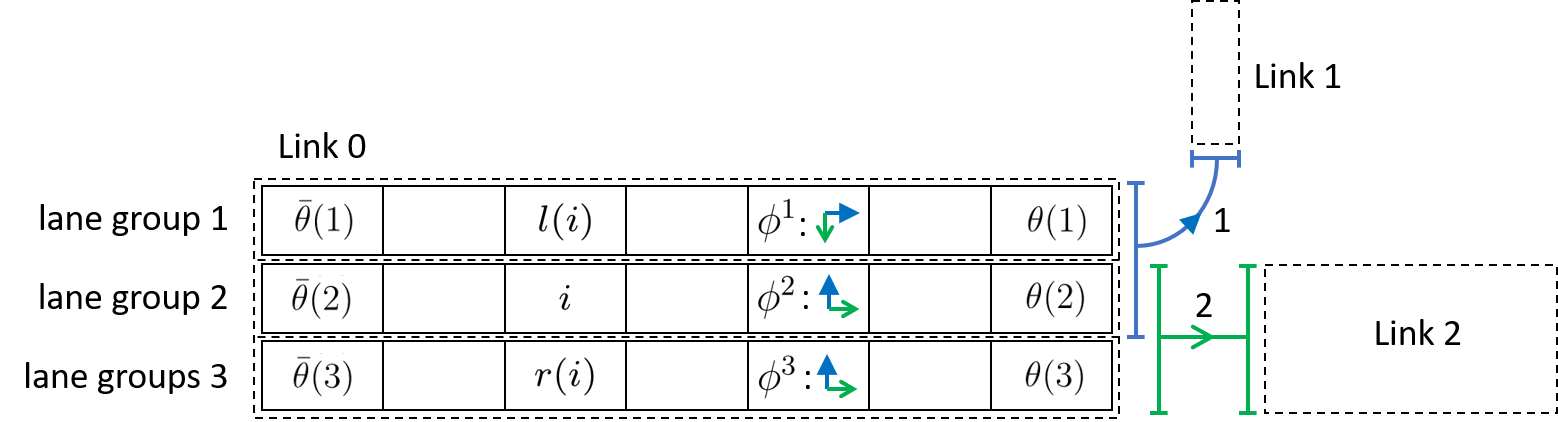
\includegraphics[width=\columnwidth]{figs/cells.png}
    \caption{CAPTION.}
    \label{fig:cells}
\end{figure}

In the CTM model of OTM, each lane group is divided into a sequence of cells, as shown in Figure \ref{fig:cells}. Vehicles are classified according to their \textit{type}. The vehicle type encodes two sets of parameters. First, it determines the vehicle's routing behavior which may be route-based or probabilistic. Route-based vehicles follow a predetermined sequence of links from their origin to their destination. Probabilistically routed vehicles direct themselves at every junction according to time-varying turning probabilities. The software supports arbirary numbers of route-based and probabilistic vehicle types. The second parameter encoded by the vehicle type is the \textit{passenger-vehicle equivalent factor}. This factor scales the size of the vehicle in the calculation of demand. For example a truck may have a passenger-vehicle equivalent factor of 3, meaning that it occupies the space of three passenger vehicles.

The state of each cell is the number of vehicles in the cell for each vehicle type and each downstream link. The downstream link of a vehicle is the next link in its route. This is determined in step XXX below for probabilistically routed vehicle types. Vehicles change lanes (ie move laterally between cells in adjacent lane groups) in order to reach a lane group that connects (via road connections) to its downstream link. 

The state update equation for each cell is executed in the following steps:

\vspace{1em} \noindent \textbf{1) Demand and supply calaculations.} The total demand and supply for every cell are computed using the standard formulas of the cell-transmission model for a triangular fundamental diagram. For the downstream-most cell in each lane group, the demands are referenced to the road connections that connect to the respective downstream links\footnote{OTM imposes the restriction that there can be at most one road connection joining a given upstream lane group to a downstream link}. Prior to computing the longitudinal demand, the model executes all lateral movements (lane changes). [XXX] provides the details. 

\vspace{1em}\noindent \textbf{2) Inter-link flow calculation.} The flows between links travel along road connections. The \textit{node model} resolves these flows from upstream demands and downstream supplies. The details of the node model can be found in XXX. Here it will suffice to state that the output of the node model is a set of \textit{state packets} that are delivered along road connections to downstream links. The node model ensures that the downstream links have sufficient available space to accomodate the state packets.  

\vspace{1em}\noindent \textbf{3) Probabilistic routing.} 
In Figure~\ref{fig:cells}, vehicles that enter link 0 must decide whether they will proceed to link 1 or link 2. This selection is made by probabilistically routed vehicles \textit{upon entering} link 0 by sampling a predifined turning probability distribution. This sampling step is carried out as state packets arrive to a link through a road connection. 

\vspace{1em} \noindent \textbf{4) State update.} Once all packets have been received and tagged with their next downstream link, then the state of the cells can be updated using the conservation of vehicles. This calculation follows the standard cell transmission model formulas for internal cells, and involves the inter-link packets for the first and last cells in a lane group. 

\subsection{Network partitioning}

The first step in the distribution of computation over $n$ processes is to split the network into $n$ overlapping subnetworks. To obtain these, the set of nodes is first partitioned into $n$ non-overlapping sets. Use $\mathcal{N}_i$, $i\in[1\hdots n]$, to denote the $i$th subset of nodes. The $i$th subnetwork contains all of the nodes in $\mathcal{N}_i$, as well as all of the links with either its start or its end node in $\mathcal{N}_i$. 
Links with start node in one subset and end node in another constitute the \textit{overlap} between two subnetworks. An overlap link with start node in $\mathcal{N}_i$ and end node in $\mathcal{N}_j$ is called a \textit{relative source} with respect to subnetwork $j$ and a \textit{relative sink} with respect to subnetwork $i$. The road connections that enter (exit) a relative source (sink) link are called \textit{relative source (sink) road connections} (with respect to a given subnetwork). The implementation includes an off-line module that invokes METIS [XXX] to create the node subsets, and then constructs separate inpute files for each of the subnetworks. These files contain all of the information (and \textit{only} that information) that is required to run the given subnetwork as a stand-alone simulation. 

\subsection{Process communication}

The connections between the $n$ subnetworks are encoded in a \textit{metagraph}. This is a graph in which each vertex represents the non-overlapping portions of a subnetwork, and the edges are the overlapping links. Each subnetwork (internal links as well as overlapping links) is managed by a separate process. The appropriate MPI communicator for this configuration is the 'graph communicator', which encodes the relations of the metagraph. An 'all-to-all' transmission with a graph communicator exchanges messages amongst neighboring vertices in the metagraph. 

The message passed between two neighboring processes consists of an array of numbers representing the vehicles that travel along all of the relative source and sink road connections that join the two subnetworks. During the initialization phase, the processes construct and exchange decoder maps with each of their neighbors. These map each position in the array to a lange group and state index. This same map is used throughout the entire simulation. The approach is conservative in the sense that the size of the message is fixed, and may contain many zeros at any given time. 

The number of vehicles that travel at each time step over road connections (i.e. the flow between links) is computed by the node model in step 2. The MPI communication step is then inserted between steps 2 and 3 from Section XXX. This completes the input and output flow computation for relative sources and sinks. After this, step 3 is executed to compute the downstream link for probabilistically routed vehicles, and then the internal state of all of the lane groups is updated. These steps are identical to their counterparts in the sequential model. Hence the result is not affected by the distribution of the calculation over multiple processes.

\section{A small example}
asdf sadf asdf asdf 




\section{Experiments}
We ran OTM simulations on a Cray XC40 Cori supercomputer at NERSC~\cite{Cori}. Each node has two sockets, each socket is
populated with a 16-core Intel\textcopyright~Xeon\texttrademark~Processor E5-2698 v3 (``Haswell'') at 2.3 GHz and 128 GB of RAM memory. This is a very modern parallel computer, taking advantage of recent technology advances in parallel computers.

\subsection{Experiment on Large-scale Synthetic Network}
\begin{figure}[h!]
    \centering
    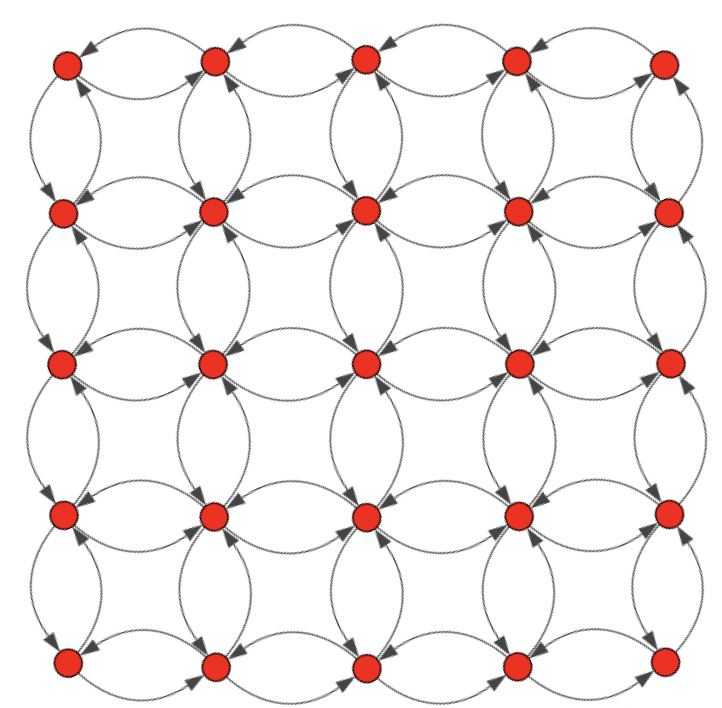
\includegraphics[height=3in]{figs/Grid-Network.png}
    \caption{Large-scale Synthetic Network with 62500 nodes and 170,000 links}
    \label{fig:Synthetic_Network}
\end{figure}

We conducted experiments on a large, grid-like, synthetic network, shown in fig. \ref{fig:Synthetic_Network}, to demonstrate the scalability of the parallel OTM in large networks. The network was composed of 62,500 nodes and 170,000 links. The traffic demand was from 12,500 origin destination pairs and the simulation was run for 1000 seconds. Fig. \ref{fig:mpirun} show the bread-down of the time used for loading and configuring the network into OTM format (load), running the simulation (run), and communication between the network partitions, as the number of processes increased from 1 to 1024. As the number of processes used for simulation increased, the size of the network partition per process also decreased. Accordingly, the time to load, simulated and communicate also decreased as each process had less computation/communication to do.

\begin{figure}[h!]
    \centering
    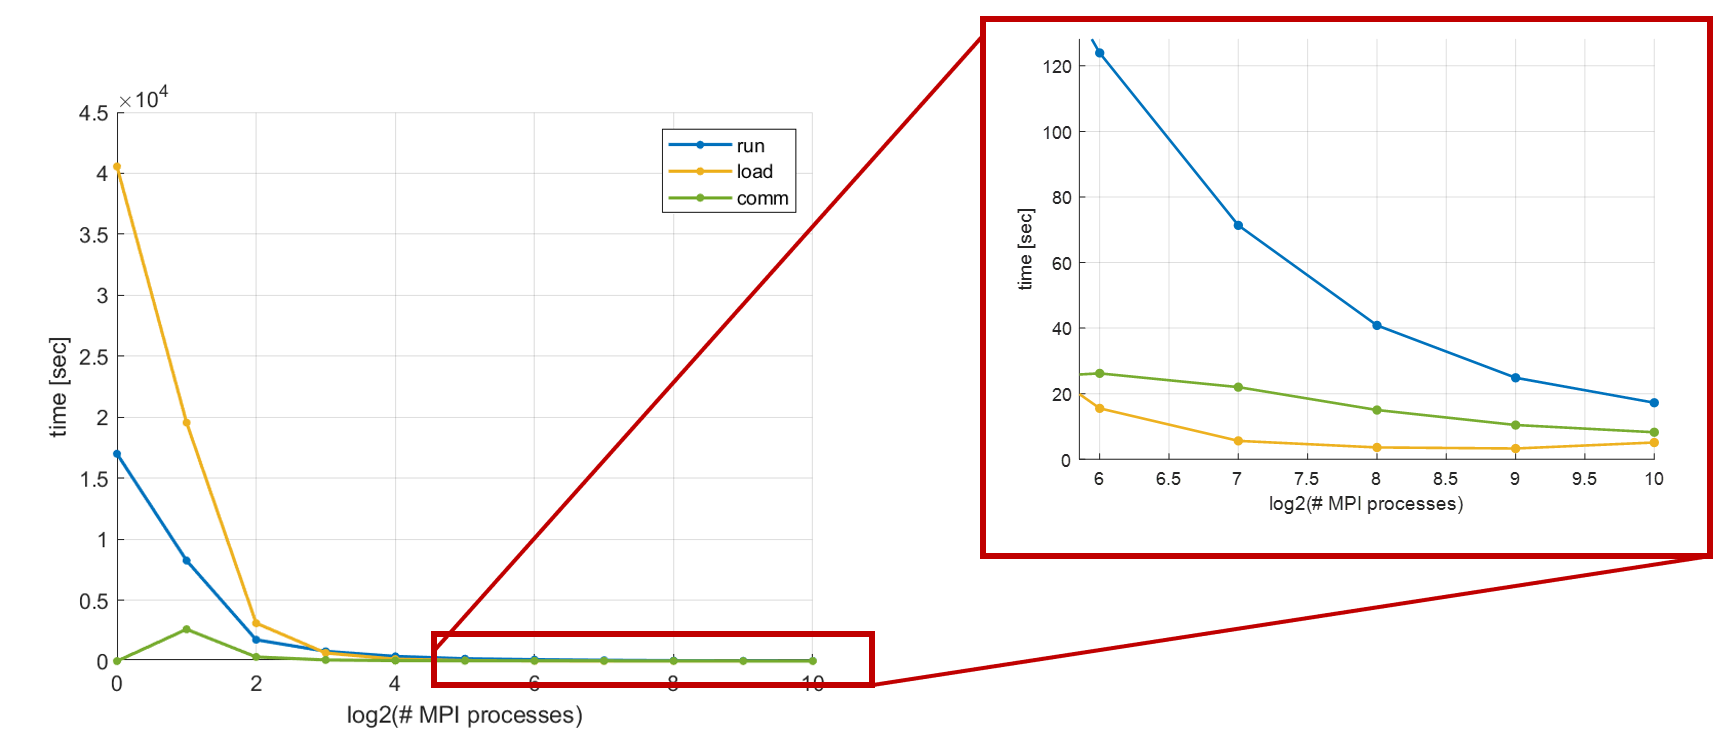
\includegraphics[width=\columnwidth]{figs/mpirun.png}
    \caption{CAPTION.}
    \label{fig:mpirun}
\end{figure}
Fig. \ref{fig:scaling} demonstrate the scaling of parallel OTM compared to the ideal scaling simulation rate. For each simulation experiment, the simulation rate $1/(simulation \:time)$, which corresponds to the number of simulations that can be completed within 1 seconds (simulations/s). The ideal rate is calculated as $(number\: of\: processes)*(serial\: simulation\: rate)$, and assumes that simulation rate increases proportionally with the number of processes. In practice, parallel simulation does not attain the ideal scaling rate as the $(communication\:time)/(simulation\:time)$ ratio grows with the number of processes. In fact, we observed that for the experiment with 1024 processes, each process spend half of its computation time in communicating with other processes. However, we still observed that for the simulation time, the parallel OTM had a speed up of 475 times with 1024 processes compared to the serial OTM. This corresponded to a time reduction from 8,245 seconds to 17 seconds.

\begin{figure}[h!]
    \centering
    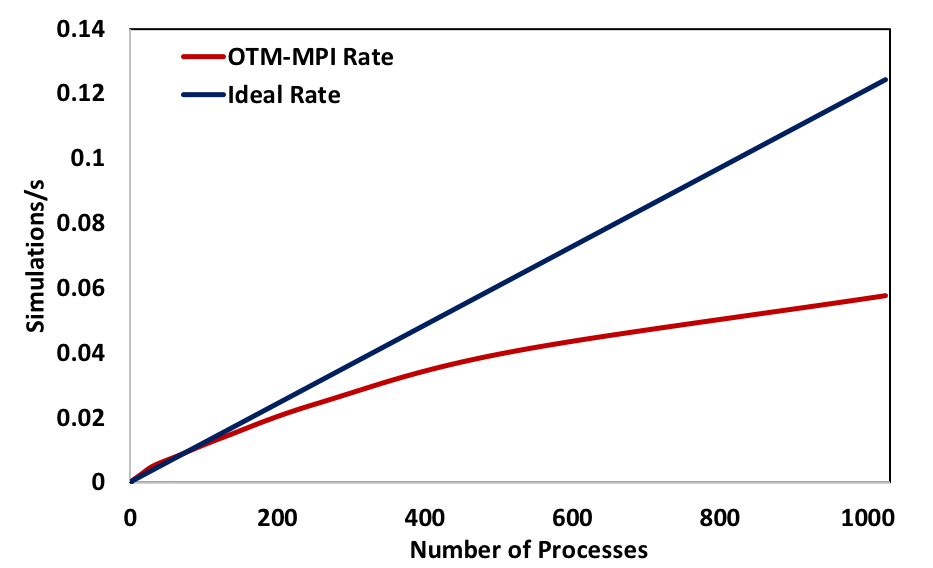
\includegraphics[width=\columnwidth]{figs/Scaling.png}
    \caption{Parallel OTM Scaling Rate compared to Ideal Scaling Rate}
    \label{fig:scaling}
\end{figure}

\subsection{Experiment on Miami Network}
We also conducted simulation experiments on a network for a section of Miami, Florida. The goal was to demonstrate how the parallel OTM scale when simulating traffic networks with realistic topology. The Miami network with $x$ nodes and $y$ links, and was extracted from OpenStreetMap\cite{haklay2008openstreetmap}. We then converted the network into OTM network format. This scenario had $z$ origin-destination pairs, and was simulated for $q$ seconds. 

We also conducted experiments to verify that the parallel OTM maintained the same traffic states as the serial OTM. We did this by comparing the vehicle density in every link and every 100 seconds between the serial simulation and parallel simulations. 

\vspace{1in}



% Network Statistics:
%     88408 nodes
% 	121946 edges



% Figure\ref{fig:chicago}


% \begin{figure}[h!]
%     \centering
%     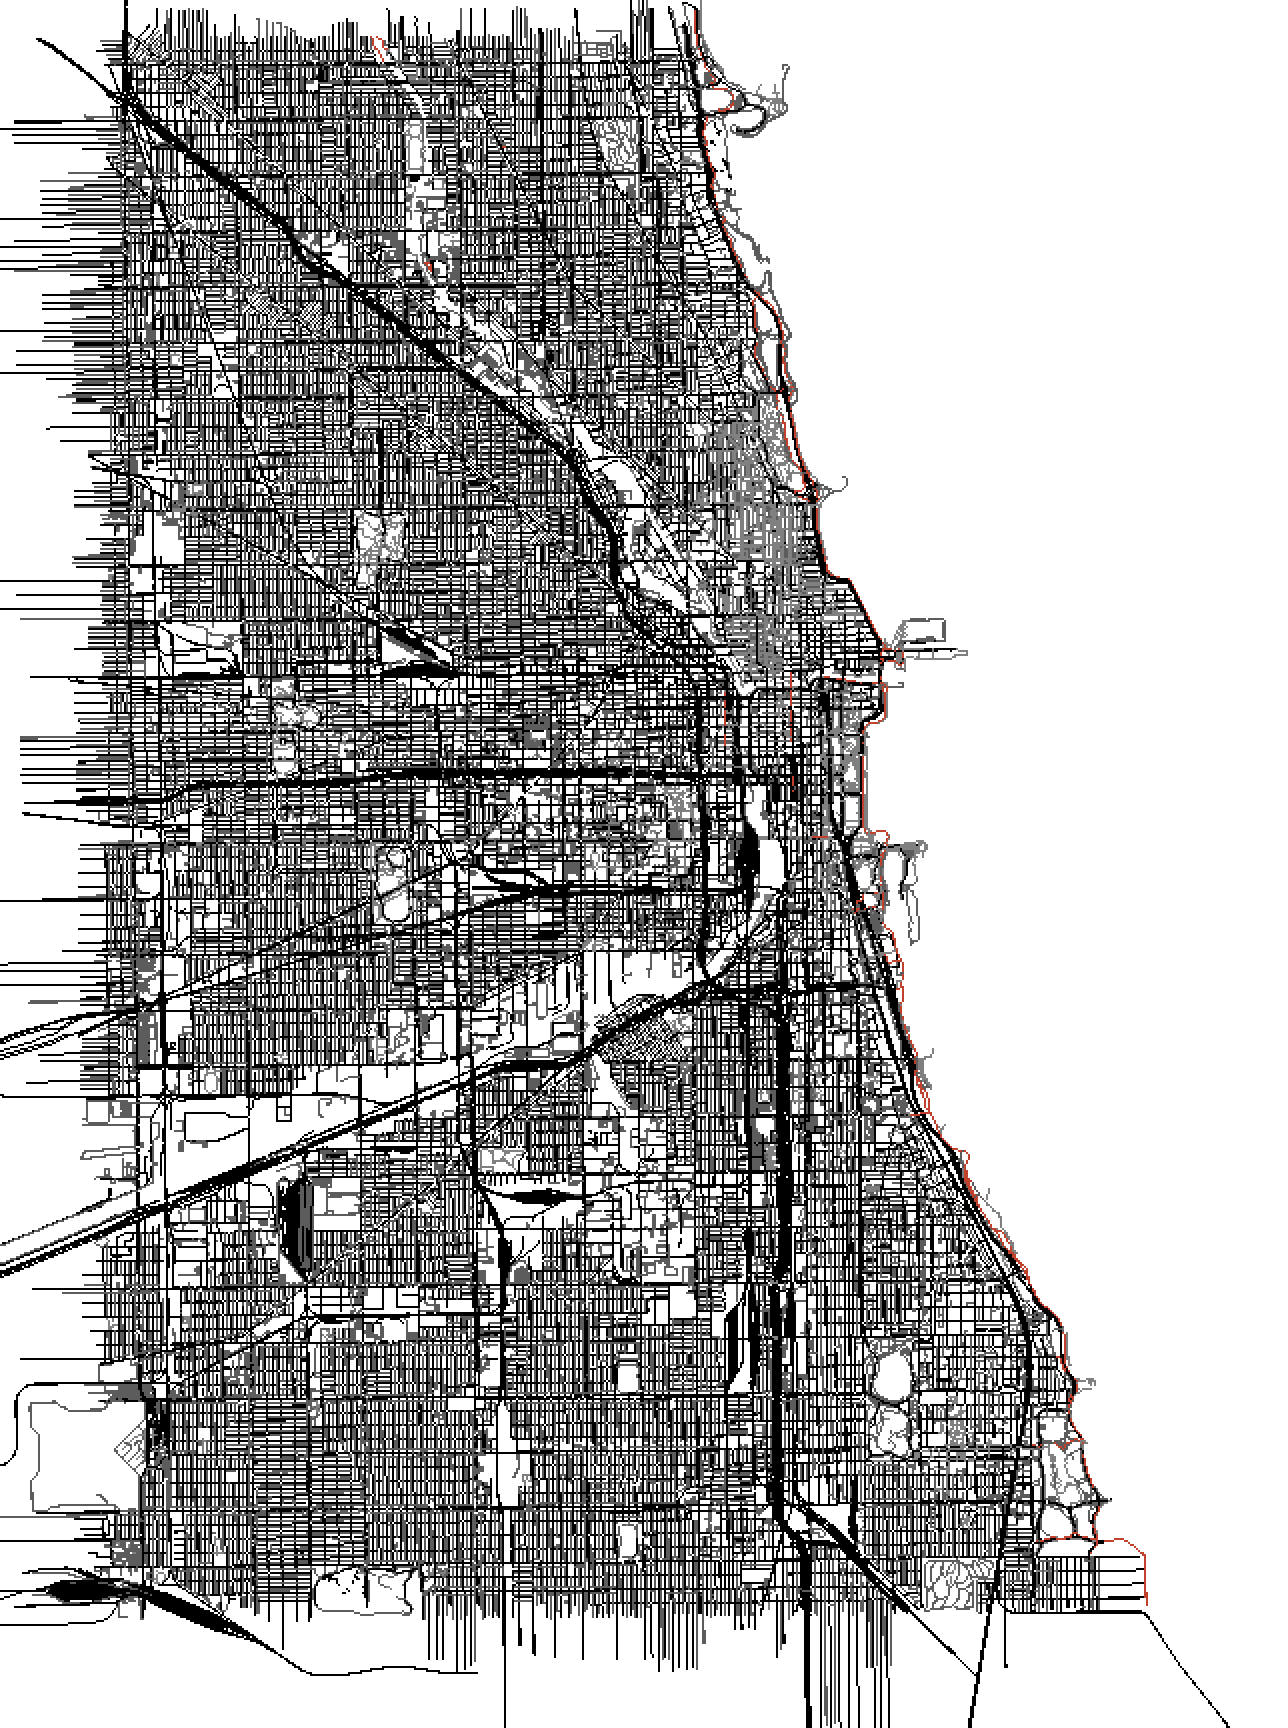
\includegraphics[height=3in]{figs/Chicago_Net_Black_White.png}
%     \caption{CAPTION.}
%     \label{fig:chicago}
% \end{figure}
 








% \subsection{Extra-Projection Method}
% The Extra-Projection method is an algorithm used to solve the dynamic user equilibrium problem. The inputs to the problem are a traffic network and a set of traffic demand $d_w : [0,T]\rightarrow \mathbb{R}^+ $, where $w\in\mathcal{W}$ is the set of origin destinations (OD) pairs. A solution $h$ is vector of demand on all available $ p\in\mathcal{P}$, where $h_p$ is the demand on path $p$. An optimal solution is a solution that creates a Wardrop traffic equilibrium \cite{wardrop1952some}. 

% EPM is based on the Euclidean projection defined as $\Pi_\mathcal{H}(x) = \underset{h}{\text{argmin}}\{\lvert h-x\rvert_2 \; : \;h \in\mathcal{H} \}$ and convergences when the travel cost function $F$ is Lipschitz continuous and pseudo-monotone. EMP has the following steps \cite{nie2010solving}:
% \begin{enumerate}
%     \item Start with an initial feasible solution $h^{1}$, set $k=1$ and set $\tau^1$ to a value less than the Lipschitz constant of $F$
%     \item Stop if $\frac {\langle c^k,y^k-h^k \rangle}{\langle y^k, c^k\rangle} \leq \epsilon$, where $c^k$ is a vector of travel cost $c_p^k$ for each path  $ p\in\mathcal{P}$ given demand $h^k$ and $y^k$ is the all-or-nothing assignment.
%     \item Determine $h^{k+1} = \Pi_\mathcal{H}(h^k - \tau^k F(z^k))$, and go back to step (2).
% \end{enumerate}

% The most time-consuming steps of the above algorithm are step 2 when calculating the all-or-nothing assignment, and steps 3 and 4 when performing the projection. This is because they involve looping over all the OD pairs, to determine the shortest path in step 2 and euclidean projection for step 3 and 4. Given $N$ computing cores, parallel computation is used to distribute the $\mathcal{W}$ od pairs among the $N$ cores such that each compute core performs step 2, 3 and 4 for $\mathcal{W}/N$ od pairs. 


\section{Conclusion}
THIS IS THE CONCLUSION


\section*{Acknowledgement}
This work is supported in part by the Office of Science of
the U.S. Department of Energy under contract No. DE-AC02-
05CH11231. 



% 
% biography section
% 
% If you have an EPS/PDF photo (graphicx package needed) extra braces are
% needed around the contents of the optional argument to biography to prevent
% the LaTeX parser from getting confused when it sees the complicated
% \includegraphics command within an optional argument. (You could create
% your own custom macro containing the \includegraphics command to make things
% simpler here.)
%\begin{IEEEbiography}[{\includegraphics[width=1in,height=1.25in,clip,keepaspectratio]{mshell}}]{Michael Shell}
% or if you just want to reserve a space for a photo:



%\vfill

\begin{IEEEbiography}{Gabriel Gomes}
Biography text here.
\end{IEEEbiography}

% if you will not have a photo at all:
\begin{IEEEbiographynophoto}{Juliette Ugirumurera}
Biography text here.
\end{IEEEbiographynophoto}

% insert where needed to balance the two columns on the last page with
% biographies
%\newpage

\begin{IEEEbiographynophoto}{Xiaoye Li}
Biography text here.
\end{IEEEbiographynophoto}


%\vfill



% Can be used to pull up biographies so that the bottom of the last one
% is flush with the other column.
%\enlargethispage{-5in}


\bibliography{_refs}{}
\bibliographystyle{IEEEtran}

\end{document}


